\documentclass[preview,border=10pt]{standalone}

\usepackage[utf8]{inputenc}				% Кодировка utf8
\usepackage[english, russian]{babel}	% Языки: русский, английский
\usepackage{amssymb,amsmath}

\usepackage{graphicx}
\usepackage[noend]{algpseudocode}

\DeclareMathOperator*{\argmax}{arg\,max}
\DeclareMathOperator*{\argmin}{arg\,min}
\renewcommand{\algorithmiccomment}[1]{{\quad\footnotesize // #1}}

\begin{document}
	\begin{center}
		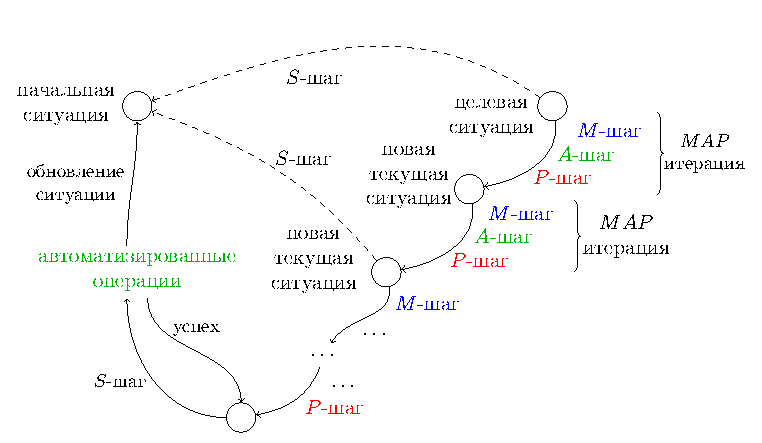
\includegraphics[width=\textwidth]{../images/algo/ru/beh_plan2_ru}
	\end{center}
	
	Алгоритм процесса планирования поведения в знаковой картине мира.
	
	\textbf{Алгоритм MAP-planner}
	\vspace*{2pt}
	\hrule
	\vspace*{1pt}
	\hrule
		
	\begin{algorithmic}[1]
		\Require описание домена планирования $D$, описание задачи планирования $P$, максимальная глубина итераций $i_{max}$
\Ensure план $Plan$

\vspace*{1pt}
\hrule
\vspace*{5pt}

\State T = $\langle N_T,S,Sit_{start}, Sit_{goal}\rangle$ := \Call{ground}{$P$}\label{alst:ground}

\Statex\Comment{$N_T$ - идентификатор задачи, $S$ - множество знаков, $Sit_{start}=\langle id_{start} \varnothing, \varnothing, \{z_{start}^a\} \rangle$ - начальная ситуация со смыслом $a_{start}$, $Sit_{goal}=\langle id_{goal} \varnothing, \varnothing, \{z_{goal}^a\} \rangle$ - целевая ситуация со смыслом $a_{goal}$}
\State $Plan$ := \Call{map\_search}{$T$}


\Function{map\_search}{$T$}
	\State $z_{cur} := z_{goal}^a$
	\State $z_{start} := z_{start}^a$
	\State $Plans$ := \Call{map\_iteration}{$z_{cur}$,$z_{start}$, $\varnothing$, 0}\label{alst:start_iter}
	\State $\{Plan_0, Plan_1,\dots\}$ = \Call{sort}{$Plans$}\label{alst:sort}
	\State\Return $Plan_0$\label{alst:return}
\EndFunction


		\Function{map\_iteration}{$z_{cur}$,$z_{start}$, $Plan_{cur}$, $i$}
	\If{$i \geq i_{max}$}\label{alst:exit}
		\State\Return $\varnothing$
	\EndIf
	
	\State $\hat A_{case}:=\varnothing$ \Comment{Список прецедентов}
	
	\Statex\Comment{$S$-этап}
	\Statex\Comment{Поиск прецедентов выполнения действий в текущих условиях}
		
	\ForAll{$s\in S$} \label{alst:check_wm}
		\ForAll{$z_a\in a(s)$}\label{alst:check_a}
			\If{$z_a \geq z_{cur}$}
				\State $\hat A_{case} = \hat A_{case} \cup \varphi_a^\uparrow(s,d_a)$ \label{alst:search_case}
			\EndIf
		\EndFor
	\EndFor
		\Statex\Comment{$M$-этап}
\Statex\Comment{Распространение активности вниз по сети личностных смыслов}
\State $A^* = \varphi_a^\downarrow(z_{cur}, d_a)$\label{alst:state_def}
\State $M^*=\varnothing$
\ForAll{$z_a\in A^*$}
	\Statex\Comment{Распространение активности вверх по сети значений}
	\ForAll{$z_m\in \varphi_m^\uparrow(s(z_a), d_m)$} \label{alst:search_act}
		\If{$I^e(z_m) \not= \varnothing$}
			\State $M^* := M^*\cup\{z_m\}$ \label{alst:add_signif}
		\EndIf
	\EndFor
\EndFor

		\Statex\Comment{$A$-этап}
\State $\hat A_{gen}=\varnothing$
\ForAll{$z_m\in M^*$}
	\Statex\Comment{Распространение активности вниз по сети значений}
	\State $\hat M^*=\varphi_m^\downarrow(z_m, d_m)$\label{alst:a_spread_m}
	\ForAll{$z_m^*\in \hat M^*$}
		\State $\hat A_{gen} := \hat A_{gen}\cup\{\Psi_m^a(z_m^*)\}$ \label{alst:a_gen_a}
	\EndFor
\EndFor
\Statex\Comment{Совмещение активности образованных смыслов и текущей ситуации}
\State $\hat A = \hat A_{gen}\cup \hat A_{case}$
\ForAll{$z_a\in \hat A$}
	\State $z_{shift}=(e_i|i\in I^e(z_a))$ \label{alst:a_shift}
	\If{$z_{cur} \not\geq z_{shift}$}
		\State $\hat A = \hat A\setminus\{z_a\}$ \label{alst:a_filter}
	\EndIf
\EndFor
\Statex\Comment{Метакогнитивная проверка эвристики}
\State $\hat A=\{\theta_a(z_a)|z_a\in\hat A\}$ \label{alst:a_meta}
\If{$\hat A = \varnothing$}
	\State\Return $\varnothing$
\EndIf

			\Statex\Comment{$P$-этап}
	\State $Plans_{fin} := \varnothing$
	\ForAll{$z_a\in\hat A$}
		\State $Plan_{cur} = Plan_{cur}\cup\{\langle z_{cur}, z_a\rangle\}$
		\Statex\Comment{Генерация новой ситуации - применение действия} 		
		\State $z_{next} := (e_i|(e_i\in z_{cur} \land e_i\not\in\{e_j|e_j\in z_a, j\in I^e(z_a)\}) \lor e_i\in\{e_k|e_k\in z_a, k\in I^c(z_a)\})$\label{alst:p_next_gen}
		\State $Sit_{next} = \langle id_{next}, \varnothing, \varnothing, \{z_{next}\} \rangle$
		\If{$z_{next} \geq z_{start}$}\label{alst:suc_exit}
			\State $Plans_{fin} = Plans_{fin}\cup\{Plan_{cur}\}$
		\Else
			\State $Plans_{rec}$ := \Call{map\_iteration}{$z_{next}$,$z_{start}$, $Plan_{cur}$, $i+1$}
			\State $Plans_{fin} = Plans_{fin}\cup Plans_{rec}$
		\EndIf
	\EndFor
	
	\State\Return $Plans_{fin}$
\EndFunction
	\end{algorithmic}

\end{document}
